\chapter{Continuous Dynamical Systems}

\section {Recap - Why we need to introduce ODEs}
As we said in the previous chapter, using a discrete representation for the steps in our model can lead us to lose all the informations that happens between the step $N_t$ and the step $N_t+1$. \par
The simplest solution is to make the distance in time $\Delta t$ between the to step very small ($\approx 0$), but it is not enough.

\section{Reconsidering the population model}
Recall in our population model that with $N(t)$ we denote the \textbf{density of some population} at time t. Our goal is to construct a mathematical model able to predict the density of the same population at a time $t^{'} = t + \Delta{t}$.

\subsection {Introducing the Ordinary Differential Equation}

\par Given our equation which is based the model:
\begin{center}
    $N(t + \Delta{t}) = N(t) + \lambda{\frac{\Delta{t}}{\sigma}{N(t)}}$
\end{center}
And the corresponding \textbf{recurrence equation}:
\begin{center}
    $N_{t+1} = r_{d}N_{t}$
\end{center}
where $r_{d} = \frac{\Delta{t}}{\sigma}$ consider the case where $\Delta{t} \rightarrow 0$. This case cannot be done using discretization, because it can lead to inaccuracies.
\par To handle the case $\Delta{t} \rightarrow 0$ we make some transformation to our equation:

\begin{center}
    $N(t + \Delta{t}) = N(t) + \lambda{\frac{\Delta{t}}{\sigma}{N(t)}} \rightarrow  \frac{N(t + \Delta{t}) - N(t)}{\Delta{t}} $
\end{center}

then by simplifying we get:

\begin{center}
    $ \frac{N(t + \Delta{t}) - N(t)}{\Delta{t}} = \frac{\lambda}{\sigma}N(t) $
\end{center}

We can recognize that the left hand side can be traced back as the \textbf{difference quotient} $\frac{f(x + h) - f(x)}{h}$, \textbf{which when taken to the limit as h approaches 0 gives the derivative of the function f}.
\par Let's consider our equation for $\Delta{t} \rightarrow 0$:

\begin{center}
    $\lim_{\Delta{t} \to 0} \frac{N(t + \Delta{t}) - N(t)}{\Delta{t}} 
    = 
    \lim_{\Delta{t} \to 0} r_{c}N(t)$
\end{center}

with $r_{c} = \frac{\lambda}{\sigma}$

Note that on the right hand side $\Delta{t}$ doesn't appear, thus we can remove the limit; the term on the left hand side is the derivative of $N(t)$, indicated as simply $\dot{N}(t)$. Thus we simply the equation as follows:

\begin{center}
    $\dot{N}(t) = r_{c}N(t)$
\end{center}

We have defined the dynamics of the system as the derivative equal to a constant multiplied by the value of the function at time $t$.\par \textbf{This equation is known as Ordinary Differential Equation (ODE)}.
\par An ODE has the following properties:
\begin{itemize}
    \item it relates the function $N$ with its derivative $\dot{N}$

    \item $t \in \mathbb{R}$, \textbf{so time is continuous}
\end{itemize}

\par We would like to use the Ordinary Differential Equation to run some simulation or to compute a general solution (like we did for the recurrence relation). 

\subsection{Using the ODE}
In some very simple case, like our linear birth model, we can find the general solution by finding a closed-form definition of $N(t)$ satisfying the equation. \textbf{A closed-form definition is one that depends only on t and some constant}. 
\par for the linear growth model a solution can be found analytically. 

\par Recall our equation:
\begin{center}
    $\dot{N}(t) = r_{c}N(t)$
\end{center}
Now let's move $N(t)$ from the right to the left hand-side of the equation:

\begin{center}
    $\frac{\dot{N}(t)}{N(t)} = r_{c}$
\end{center}
Recall that $\frac{\dot{N}(t)}{N(t)} = \ln{N(t)}$ and $r_{c}$ is the derivative of $r_{c}t + c$ for any constant $c$, obtaining:

\begin{center}
    $\ln{N(t)} = r_{c}t + c$
\end{center}
By resolving our equation in regards to $N(t)$ we finally get:
\begin{center}
    ${N(t)} = Ce^{r_{c}t + c}$
\end{center}
where $C = e^{c}$ (typically $C$ is set to be equal to $N(0)$

\begin{figure}[h]
    \centering
    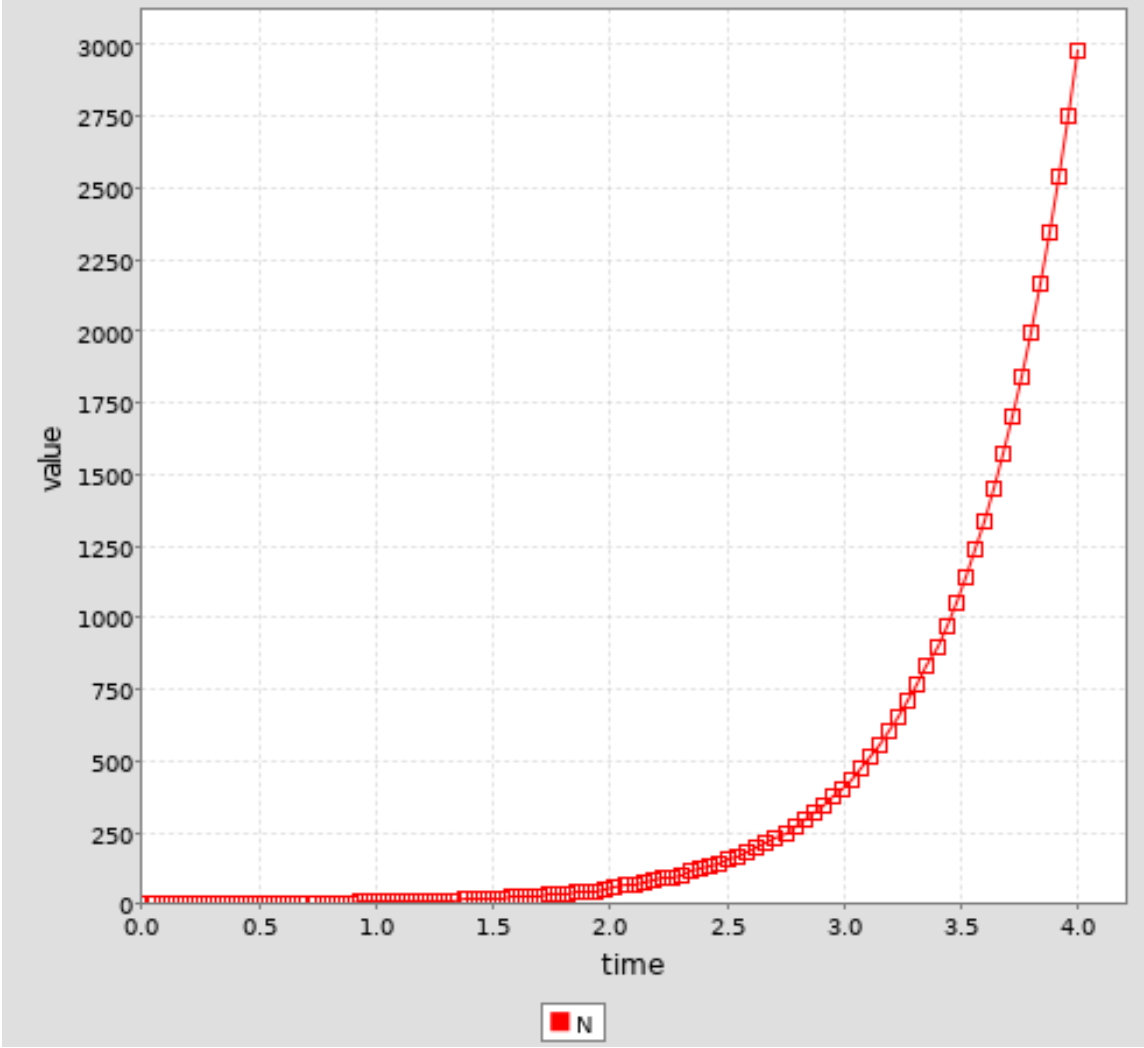
\includegraphics[width=0.5\textwidth]{Images/03 - Contiguous Dynamicsl System/linear_birth_model_continuous.png}
    \caption{This graphs shows us that by setting in our population model $r_{c} = 2$ and $C = N(0) = 1$ then the population shows an exponential growth over time.} 
\end{figure}

\subsubsection{Differences between discrete and continuous model}
This behaviour is qualitatively the same as for the discrete model, both showing exponential growth.
\textbf{What changes is the meaning of the equation}: 
\begin{itemize}
    \item the recurrence relation tells you how to update the variable.

    \item in our new equation it defines the derivative, \textbf{meaning how fast it's changing}.
\end{itemize}
Note how both equations show rate $\geq 1$ only if the birth rate $\frac{\lambda}{\sigma}$ is $\geq 1$.

\section{Example - Radioactive decay}
We move from the example of the population model we have seen so far to another one.
\par Radioactive decay is a process where we have a negative evolution of the population. The idea is that \textbf{each molecule decays at a constant rate}, so the whole mass decreases with a rate which is proportional to the mass itself.
\par We can describe this model by using the following Ordinary Differential Equation:

\begin{center}
    $\dot{N}(t) = -d_{c}N(t)$
\end{center}
then if we solve it in regards to $N(t)$ we get:
\begin{center}
    $N(t) = N(0)e^{-d_{c}t}$
\end{center}

\begin{figure}[h]
    \centering
    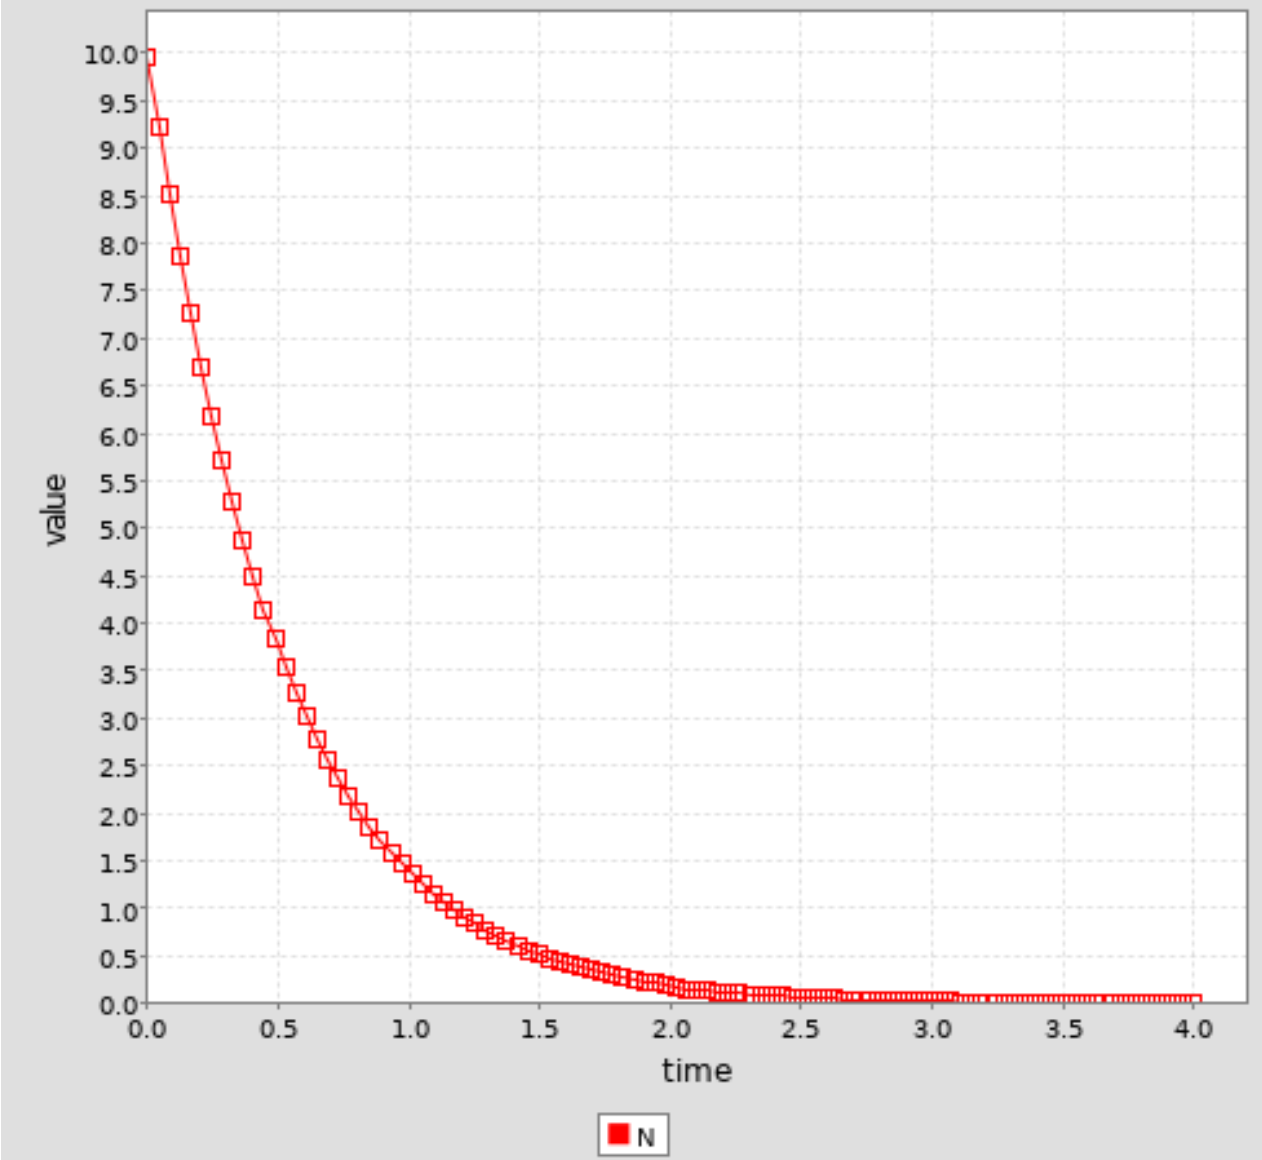
\includegraphics[width=0.5\textwidth]{Images/03 - Contiguous Dynamicsl System/Radioactive_decay.png}
    \caption{Example of applying the ODE of the radioactive decay. Note that  by setting $d_{c} = 2$ and $C = N(0) = 10$ we get $N(t)$ to tend to zero. This is caused by the negative exponent in the ODE.} 
\end{figure}

\section{Continuous version of the logistic equation}
Given the non-linear logistic equation, we can define as follows its continuous version:
\begin{center}
    $\dot{N}(t) = r_{c}N(t)(1 - \frac{N(t)}{K})$
\end{center}
where:
\begin{itemize}
    \item $r_{c}$ is the \textbf{continuous growth rate}.

    \item $K$ is the \textbf{carrying capacity} of the environment.
\end{itemize}

Resolving the ODE in regards to $N(t)$ we get:
\begin{center}
    $N(t) = \frac{K}{1 + (\frac{K}{N(0)} - 1) e^{-r_{c}t}}$
\end{center}
We notice that when $N(t) \rightarrow K$ \textbf{the population converges to the carrying capacity of the environment}.

\begin{figure}[h]
    \centering
    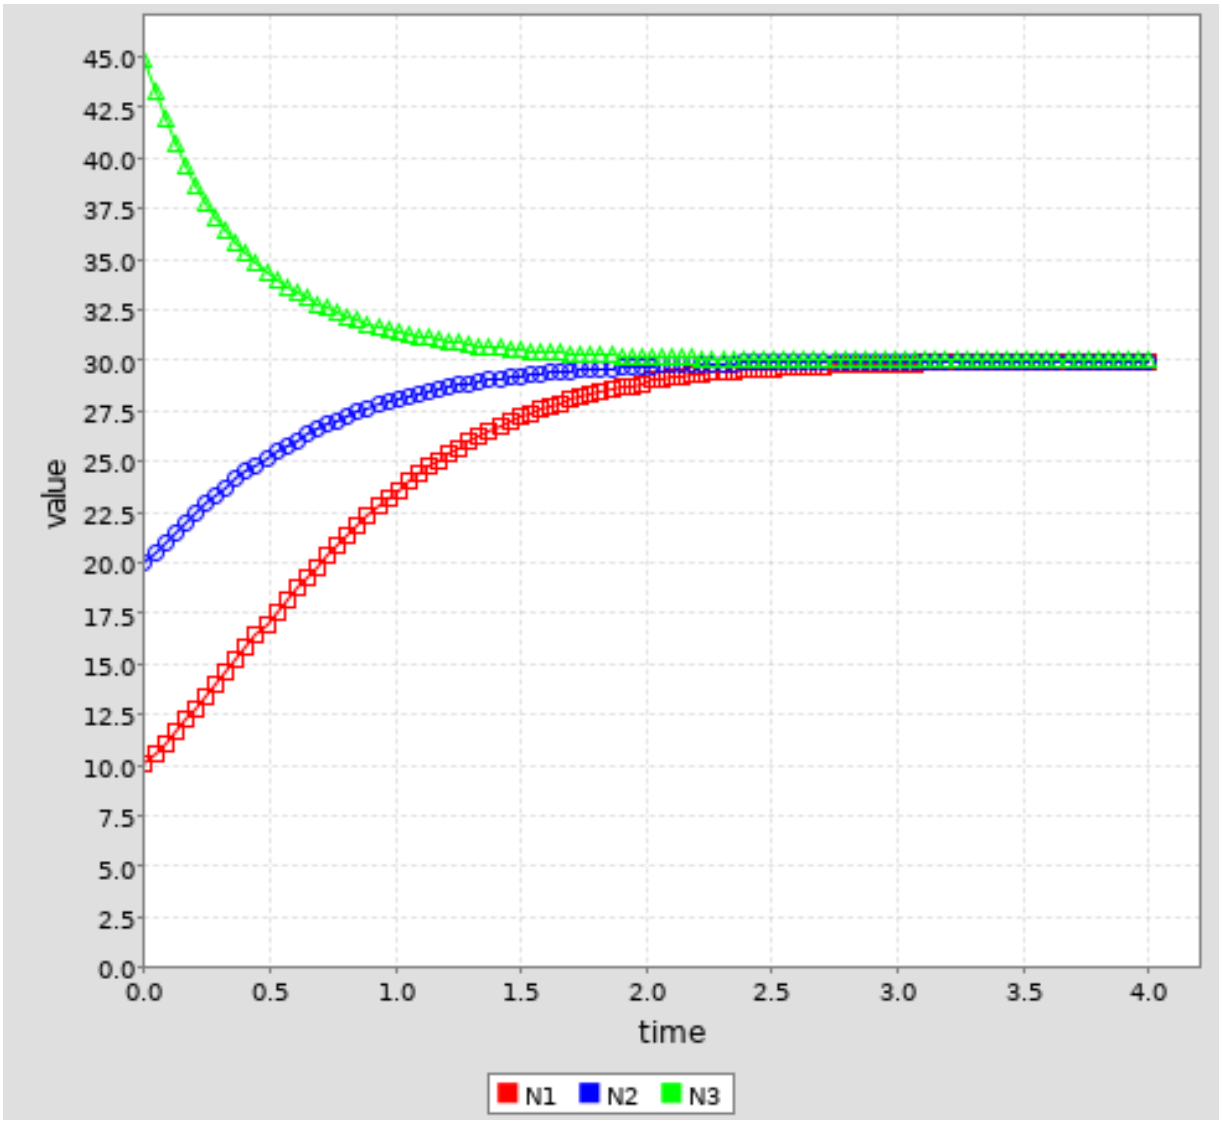
\includegraphics[width=0.5\textwidth]{Images/03 - Contiguous Dynamicsl System/continuous_logistics.png}
    \caption{Example of the continuous logistic equation. Note how by putting $r_{c} = 2$, $N(0) = 10$, $K = 30$, the population will eventually converge to the carrying capacity of the environment.} 
\end{figure}

\par \textbf{The trend is the same as for the discrete case}.

\section{Systems of ODE}
Now let's consider a population of males, indicated as $M(t)$, and females, indicated as $F(t)$. Assume that males fight with each other, so a small part of them dies because of it with a death rate of $s_{c}$. 
\par Thus we have to expand our model considering a system of ODEs:
\[
\begin{cases}
    \begin{aligned}
        \dot{F}_{t} = r_{c}F_{t}(1 - \frac{F_{t} + M_{t}} {K}) \\
        \dot{M}_{t} = r_{c}F_{t}(1 - \frac{F_{t} + M_{t}}{K}) - s_{c}M_{t}\\
    \end{aligned}
\end{cases}
\]
where:
\begin{itemize}
    \item $r_{c}F(t)$ is used for both genders, \textbf{since both are generated by females}.
    \item $F(t) + M(t)$ describes the whole population size.
\end{itemize}

\begin{figure}[h]
    \centering
    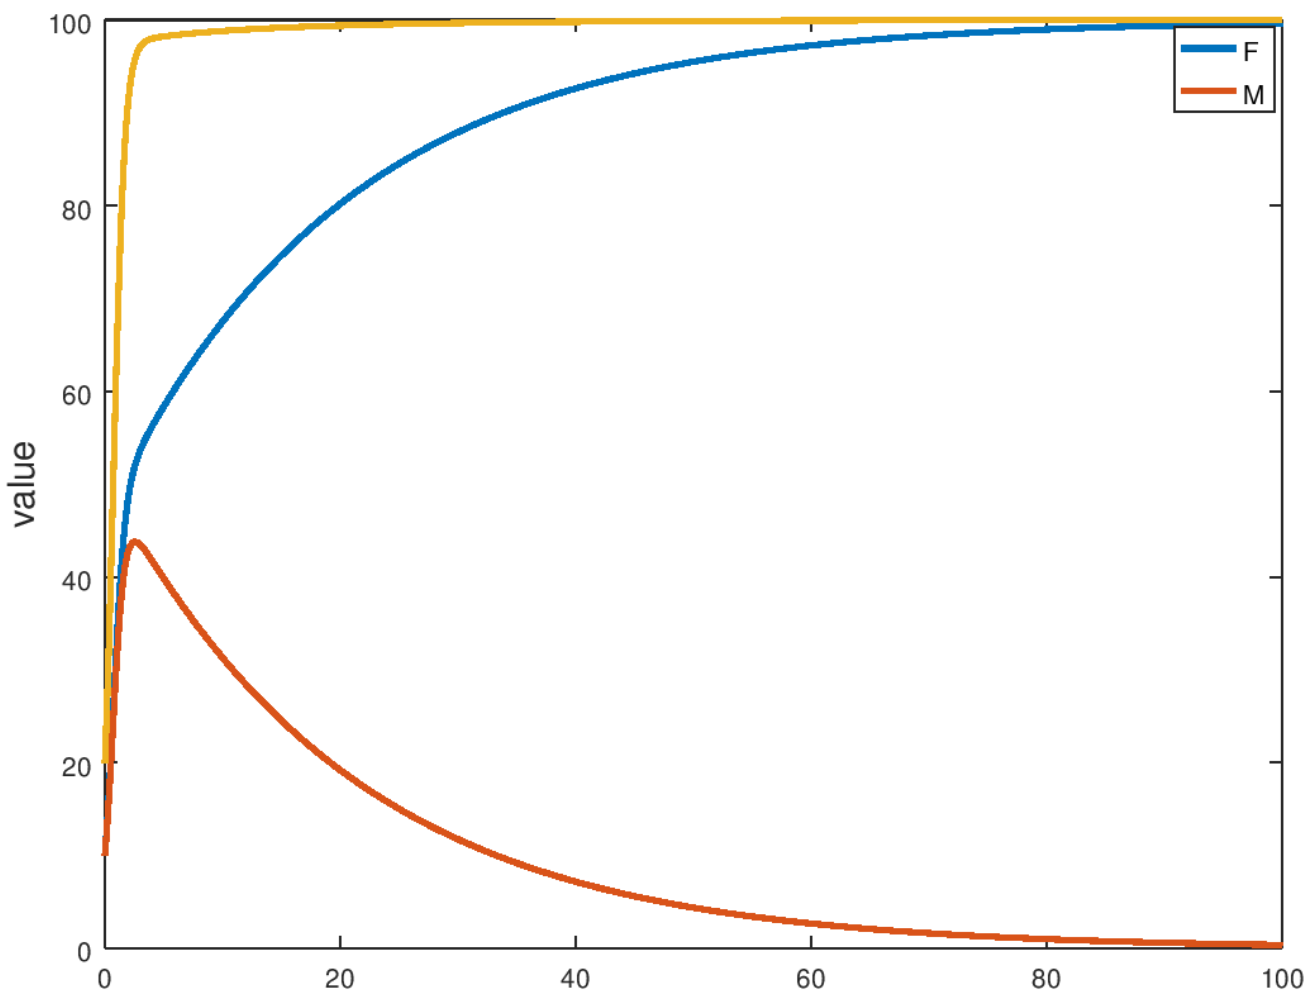
\includegraphics[width=0.5\textwidth]{Images/03 - Contiguous Dynamicsl System/system of ODE.png}
    \caption{Example of the system of ODEs.} 
\end{figure}

What happens in this scenario, after some times you have only females in the population. This shows a completely different behaviour from the discrete case, \textbf{because the meaning of their equations is different}:
\begin{itemize}
    \item The recurrence relations indicates us the size of the population.

    \item The system of ODEs describes how fast is changing.
\end{itemize}

\section{Numerical Solution of ODEs}
Recall that we said that computing the solution of an ODE is not always possible. For this reason we prefer working using an approximation of the solution, indicated as \textbf{numerical solver} (or numerical simulator). This approximation doesn't compute the general function, \textbf{instead it solves the initial value problem, also called Cauchy problem}.

\begin{center}
\subsubsection{Initial Value Problem}
Given an ODE in the form $\dot{N}(t) = f(N(t)) $ and an initial value $N_{0}$ s.t. $N(0) = N_{0}$, compute a function $F(t)$ that is a solution of the ODE and s.t. $F(0) = N_{0}$.
\end{center}

In our case we are interested only in studying the values of $F(t)$ where $t \geq 0$, \textbf{hence we perform a numerical simulation starting at} $t = 0$.

\section{The Euler method}
The Euler method is the simplest numerical simulation method available. The main concept behind this approach is to approximate the given continuous system with a recurrence relation specifically designed to approximate the continuous differential equation. \textbf{The idea is that, since we know the derivative, we use it as it was the function}.\par
It is based on the idea of discretizing the dynamics of differential equations by time steps of constant length $\tau = \Delta t$.\par
Given an Ordinary Differential Equation in the form:

\begin{center}
$\dot{N}(t) = f(N(t))$ 
\end{center}
this corresponds to approximating its solution with the following recurrence relation (assuming $N_0 = N(0)$) 
\begin{center}
$N_{k+1} = N_k + \tau f(N_k)$ 
\end{center}
where $N_k \approx N(\tau k)$

\begin{figure}[h]
    \centering
    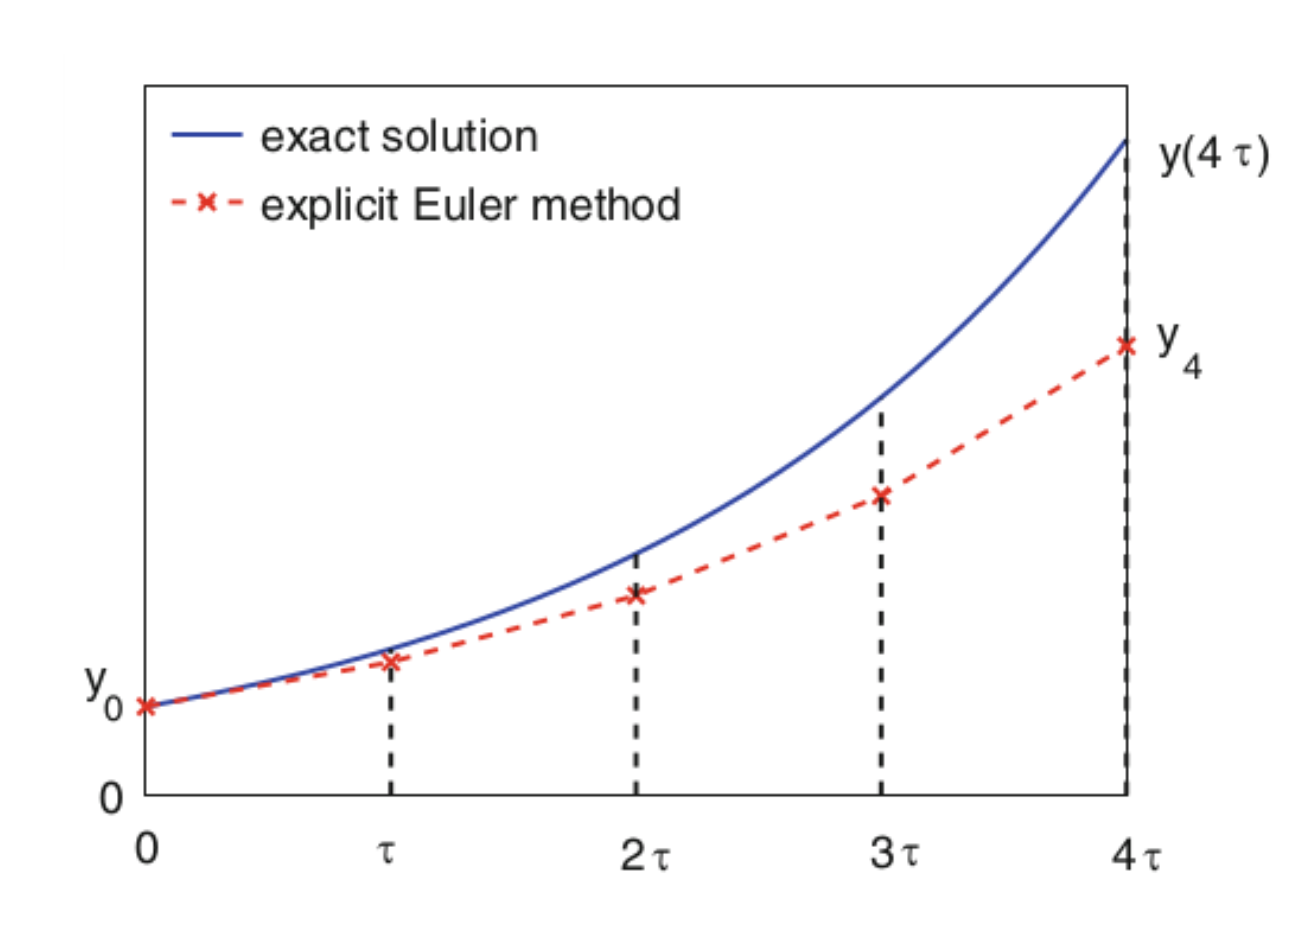
\includegraphics[width=0.5\textwidth]{Images/03 - Contiguous Dynamicsl System/Euler_method.png}
    \caption{A graph showing the correct solution compared to the approximation generated by the Euler method.} 
\end{figure}

\subsection{Errors in the Euler method}
By approximating in each step the Euler method makes local errors that will contribute to a global error at the end of the whole simulation.\par

\textbf{The local discretization error} is computed as $| N(\tau) - N_1|$ and it is in the order of $O(\tau^2)$ \textit{(the motivation is because we truncate the Taylor Series at the first step)}.\par

\textbf{The Global discretization error} is obtained by accumulate all the local discretization errors after $k$ steps, namely at time $t = k \tau$. The global error is computes as $|N(k \tau) - N_k)$ and is in the order $O(k \tau^2) = O(\tau)$ since $k \tau = t$ is constant.

\section {Other numerical simulation methods}
A linear error of $O(\tau))$ is quite annoying, requiring us to set $\tau \approx 0$ in order to have something acceptable, making the computation very slow (it requires a lot of steps).\par
To overcome this other methods have been proposed, having a global discretization error of a higher order (e.g. $O(\tau^p)$ for some p) which is better as long as $\tau \rightarrow 0$ (hence $\tau < 1$). To work these method use more than one point to approximate the value of the function, making a single step require more time, but maintain the error inside some defined boundaries. \par

A few examples of such methods are:
\begin{itemize}
    \item \textbf{Runge-Kutta methods:} $p = 2$ in the original formulation, but can be higher
    \item \textbf{Multistep methods (e.g. Adams methods):} extrapolate the value of the next step from the values of the previous k steps obtaining $p \approx k$.
\end{itemize}

State-of-art methods can also:
\begin{itemize}
    \item \textbf self-determine the step size $\tau$ based on thresholds on local and global discretization errors.
    \item \textbf dynamically adjust the step size $\tau$ during their executing (e.g. Adaptive Runge-Kutta) 
\end{itemize}

\section{Instability and stiff systems}
There is another problem that could arise: if you have a derivative which cause the value of a variable in a very fast way, if $\tau$ is not small enough you not only pay some error but you could have that your computed solution is unstable.\par
What we mean for unstable is that we lose informations and your points start to oscillate creating chaos.\par

\begin{figure}[h]
    \centering
    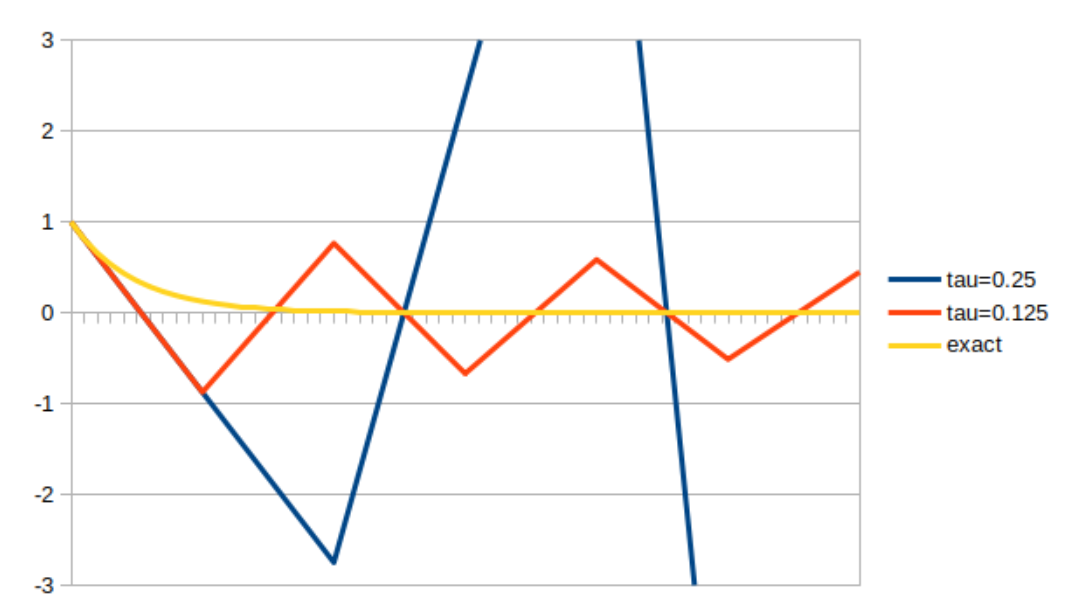
\includegraphics[width=0.5\textwidth]{Images/03 - Contiguous Dynamicsl System/Stiff System.png}
    \caption{An example of a stiff system. In orange is shown the real solution, while in red and blue the one obtained by setting $\tau$ to different values} 
\end{figure}

This kind of problematic systems are called \textbf{stiff systems}. There is no clear definition of stiffness: intuitively contains a very fast term that cannot be captured by our method, worse if we have in our systems also slow terms to take into account. \par
In this cases you need to consider alternative numerical simulation methods called \textbf{implicit numerical simulation methods}. All the methods we have seen so far have and implicit version, which requires more computation time for step.

\section{Implicit Euler method}
The idea of the implicit version of the Euler method is that, like the previous version we approximate the function by using its derivative, \textbf{but the derivative is not computed on the value $N$ at step $k$, but at the step $k+1$}.\par
By using this approach we are no longer defining $N_{k+1}$ in terms of $N_k$, but as an equation where $N_{k+1}$ is in both sides:

\begin{center}
    $N_{k+1} = N_{k} + \tau f (N_{k+1})$
\end{center}
where $N_k \approx N(k \tau)$.\par

There are methods from numerical analysis that are able to solve these type of equations. This method requires more effort for computing a single step, but \textbf{often} the local discretization error is smaller permitting us to use greater values of $\tau$.

\section{Other implicit methods}
Implementations of implicit methods that use more than one variables require the modeler to provide the \textbf{Jacobian matrix} (partial derivatives) of the function f. Most are able to compute the Jacobian matrix autonomously by doing some approximation. \par
There exist methods that are able to automatically switch from explicit to implicit methods by determining if the system is stiff.




